% !TeX spellcheck = ru_RU
% !TEX root = vkr.tex

Данный раздел посвящен описанию проводимого экспериментального исследования. В предыдущих главах были представлены основные подходы к исполнению запросов с регулярными ограничениями, а также описан новый алгоритм, основанный на операциях линейной алгебры и поиске в ширину. Сравнение производительности этого алгоритма с реализациями других подходов является основной целью данного исследования.

\subsection{Исследовательские вопросы и метрики}

В качестве основной метрики производительности рассматривается время работы алгоритмов на регулярных запросах.
Цель экспериментального исследования --- ответить на два исследовательских вопроса:

\begin{itemize}
    \item \textbf{RQ1}: Какова производительность разработанного алгоритма по сравнению с существующими аналогами?
    \item \textbf{RQ2}: Как влияет размер множества стартовых вершин на производительность реализации разработанного алгоритма?
\end{itemize}

\subsection{Окружение и конфигурации}

Экспериментальное исследование проводится на сервере под управлением ОС Ubuntu 20.04 со следующими характеристиками: процессор Intel Core i7-6700 CPU, 4 ядра с частотой 3.40 ГГц; объем оперативной памяти 64 Гб.

Для проведения сравнения с аналогом на основе языка Datalog было принято решение использовать язык Souffle~\cite{souffle}, который является одним из диалектов языка Datalog и преодолевает некоторые ограничения классического варианта. Souffle часто используется в задачах языкового анализа и имеет сейчас большую популярность. Установлена версия Souffle 2.4, которая была сконфигурирована с размером слова для примитивного типа 64 бита и запускалась с флагами \verb|-j {число ядер процессора}|, который используется для параллельного исполнения программы, и \verb|--magic-transform=*| для преобразования программы в эквивалентную с потенциально меньшим числом промежуточных вычислений.

Для подхода, основанного на построении индекса, была найдена реализация\footnote{Repository for the prototype code for index RPQ paper: \href{https://github.com/darroyue/Ring-RPQ}{https://github.com/darroyue/Ring-RPQ} (accessed: 20.05.2023)}, находящаяся в свободном доступе, которую автору удалось запустить, однако этот инструмент выдает неверный результат при запуске на сгенерированных по шаблонам запросах, по этой причине он был не включен в сравнительный анализ.

Реализация тензорного алгоритма для нескольких стартовых вершин была взята из репозитория CFPQ\_PyAlgo\footnote{Repository for developing, testing and benchmarking CFPQ algorithms implemented in PyGraphBLAS: \href{https://github.com/FormalLanguageConstrainedPathQuerying/CFPQ_PyAlgo}{https://github.com/FormalLanguageConstrainedPathQuerying/CFPQ\_PyAlgo} (accessed: 20.05.2023)}.

\subsection{Условия эксперимента}

В качестве исходных данных были выбраны графы, собранные по реальным RDF данным и данным социальных сетей. Их характеристики представлены в таблице. В таблице выделено количество вершин и рёбер графа, а также, число уникальных меток, содержащихся на рёбрах. Графы класса RDF расположены в первой части таблицы, графы социальных сетей --- во второй.

\definecolor{lightgray}{gray}{0.9}
\begin{table}[!ht]
    \centering
    \rowcolors{1}{}{lightgray}
    \begin{tabular}{|c|c|c|c|}
        \hline
        Graph      & \#V       & \#E        & \#L \\ \hline \hline
        enzyme     & 48 815    & 86 543     & 14  \\
        eclass     & 239 111   & 360 248    & 10  \\
        go         & 582 929   & 1 437 437  & 47  \\
        geospecies & 450 609   & 2 201 532  & 158 \\
        taxonomy   & 5 728 398 & 14 922 125 & 21  \\
        \hline
        advogato   & 6 541     & 51 127     & 3   \\
        youtube    & 15 088    & 27 257 790 & 5   \\
        \hline
    \end{tabular}
    \caption{Графы.}
\end{table}

Стоит отметить, что графы, собранные по данным социальных сетей являются достаточно плотными в сравнении с графами, построенными по RDF-данным, так как имеют существенно большее число ребер, чем вершин. Это может привести к тому, что во время обхода этих графов будут пройдены более длинные пути, что может сказаться на времени исполнения алгоритмов.

Регулярные запросы к графам были сгенерированы на основе самых популярных шаблонов запросов, собранных в  работе~\cite{related_oneforall}. В запросы входят классические операторы регулярных выражений такие, как конкатенация и перечисление, а также звезда Клини и множество комбинаций этих операторов. Всего отобрано 16 шаблонов, они представлены в таблице~\ref{table:queries}.

\begin{table}[!ht]
    \centering
    \rowcolors{1}{}{lightgray}
    \begin{tabular}{|c|c||c|c|}
        \hline
        Name  & Query                           & Name     & Query                                           \\ \hline \hline
        $q_0$ & $a^*$                           & $q_{8}$  & $a \cdot b$                                     \\
        $q_1$ & $a \cdot b^*$                   & $q_{9}$  & $a \cdot b \cdot c$                             \\
        $q_2$ & $a \cdot b^* \cdot c^*$         & $q_{10}$ & $a \cdot b \cdot c \cdot d$                     \\
        $q_3$ & $a \cdot b^* \cdot c$           & $q_{11}$ & $(a \cdot b)^+~|~(c \cdot d)^+$                 \\
        $q_4$ & $a^* \cdot b^*$                 & $q_{12}$ & $(a \cdot (b \cdot c)^*)^+~|~(d \cdot e)^+$     \\
        $q_5$ & $a \cdot b \cdot c^*$           & $q_{13}$ & $(a \cdot b \cdot (c \cdot d)^*)^+~|~(e~|~f)^*$ \\
        $q_6$ & $(a~|~b~|~c~|~d~|~e)^+$         & $q_{14}$ & $(a~|~b)^+~(c~|~d)^+$                           \\
        $q_7$ & $(a~|~b~|~c~|~d~|~e) \cdot f^*$ & $q_{15}$ & $a \cdot b \cdot (c~|~d~|~e)$                   \\
        \hline
    \end{tabular}
    \caption{Шаблоны запросов.}\label{table:queries}
\end{table}

Для каждого графа отбиралось 5 самых популярных меток, после чего по ним на основе шаблонов генерировалось случайным образом 5 запросов. Важно отметить, что в графе $advogato$ меньше 5 различных меток, по этой причине в сгенерированных для этого графа запросах допускается повторение меток.

В зависимости от числа вершин, на которых запускаются регулярные запросы, их можно разделить на несколько видов:
\begin{itemize}
    \item Single-source запросы, для которых алгоритм запускается от одной исходной вершины.
    \item Multiple-source запросы запускаются от определенного изначально множества вершин в графе.
    \item All-pairs запросы запускаются от множества всех вершин графа.
\end{itemize}

Для выбора множества начальных вершин было решено создавать случайные выборки из нужного числа вершин. Так, для single-source запросов создавалось множество из 100 начальных вершин, для каждой из которых запускался запрос. Для multiple-source запросов создавалась выборка из 2, 5, 10, 100, 1000, 10000 случайных вершин для каждого графа, на которой запускались запросы. При этом финальными считались все вершины графа. Скрипты для создания запросов и генерации вершин доступны в репозитории\footnote{Benchmark suite for RPQ evaluation:~\href{https://github.com/bahbyega/paths-benchmark}{https://github.com/bahbyega/paths-benchmark}~(accessed: 20.05.2023)}.

\subsection{Результаты сравнения алгоритмов}
\textbf{RQ1}: Какова производительность разработанного алгоритма по сравнению с существующими аналогами?

На рисунках 3--4 представлены результаты эксперимента по сравнению производительности алгоритмов на графах, построенных по RDF данным. Введены следующие обозначения: алгоритм, основанный на поиске в ширину, обозначен MSBFS, алгоритм, основанный на тензорном произведении --- Tensor, решение, основанное на Datalog и реализованное с помощью диалекта Souffle --- Datalog. Для всех шаблонов в виде гистограмм представлено среднее арифметическое значение времени исполнения алгоритмов с отклонением от среднего на соответствующем запросе.

Прежде всего эксперимент был поставлен на графах наименьшего размера --- \textit{enzyme} и \textit{eclass} для случая single-source запросов, который представлен в первой колонке. Результаты показывают, что реализации алгоритмов в терминах матричных операций в среднем на порядок быстрее реализации на Datalog. В частности, алгоритм на основе тензорного произведения работает более чем в 10 раз быстрее аналога на Datalog, алгоритм MSBFS --- в среднем в 100 раз быстрее. Важно отметить, что программы для аналога на Datalog генерировались по соответствующим представлениям регулярных ограничений в виде грамматик. Реализовать каждый из запросов для конкретного графа можно эффективнее, используя дополнительные средства языка Souffle, что могло повлиять на показатели времени, представленные на рисунках.

Далее, три реализаций запускались на multiple-source запросах. Результаты для наибольшего из множеств начальных вершин (10000 вершин) представлены на рисунках 3--4 во второй колонке. На множестве из 10000 стартовых вершин Tensor и Datalog показывают близкую производительность, проигрывая MSBFS. При этом показатели времени исполнения тензорным алгоритмом имеют более высокое отклонение от среднего значения. Это может объясняться тем, что конкретный шаблон представлен несколькими запросами с метками, расположенными в разном порядке. Из-за чего результат исполнения запроса может сильно отличаться по количеству достижимых вершин. Так, для шаблонов $q_6$, $q_8$, $q_9$, $q_{10}$ большое значение имеет порядок, в котором расставлены метки в шаблоне, потому что в них отсутствует оператор звезды Клини.

После чего проводился эксперимент на графе \textit{go}. Из него видно, что производительность MSBFS оказалась незначительно хуже алгоритма, основанного на тензорном произведении. Это может быть объяснено структурой графа \textit{go}. Он имеет большое число ребер с одной и той же меткой, которая чаще всего встречалась в запросах, что повлияло на количество шагов алгоритма MSBFS.

По экспериментам на графах \textit{geospecies} и \textit{taxonomy} также можно выделить лучшую производительность MSBFS и Tensor относительно Datalog. Однако тензорный алгоритм демонстрирует выбросы на некоторых запросах, когда запрос запускается на множестве из 10000 вершин. Кроме того, важно отметить, что производительность алгоритмов зависит от сложности запроса. Так, запросы $q_7$ и $q_{13}$, содержащие в себе большее количество меток и операторов, чем остальные запросы, исполняются в среднем дольше остальных.

% !TeX spellcheck = ru_RU
% !TEX root = vkr.tex

\newcolumntype{C}{ >{\centering\arraybackslash} m{4cm} }
\newcommand\myvert[1]{\rotatebox[origin=c]{90}{#1}}
\newcommand\myvertcell[1]{\multirowcell{5}{\myvert{#1}}}
\newcommand\myvertcelll[1]{\multirowcell{4}{\myvert{#1}}}
\newcommand\myvertcellN[2]{\multirowcell{#1}{\myvert{#2}}}

\afterpage{
    \clearpage
    \thispagestyle{empty}
    \begin{landscape}
        \centering
        \begin{figure}
            \begin{tabular}{cc}
                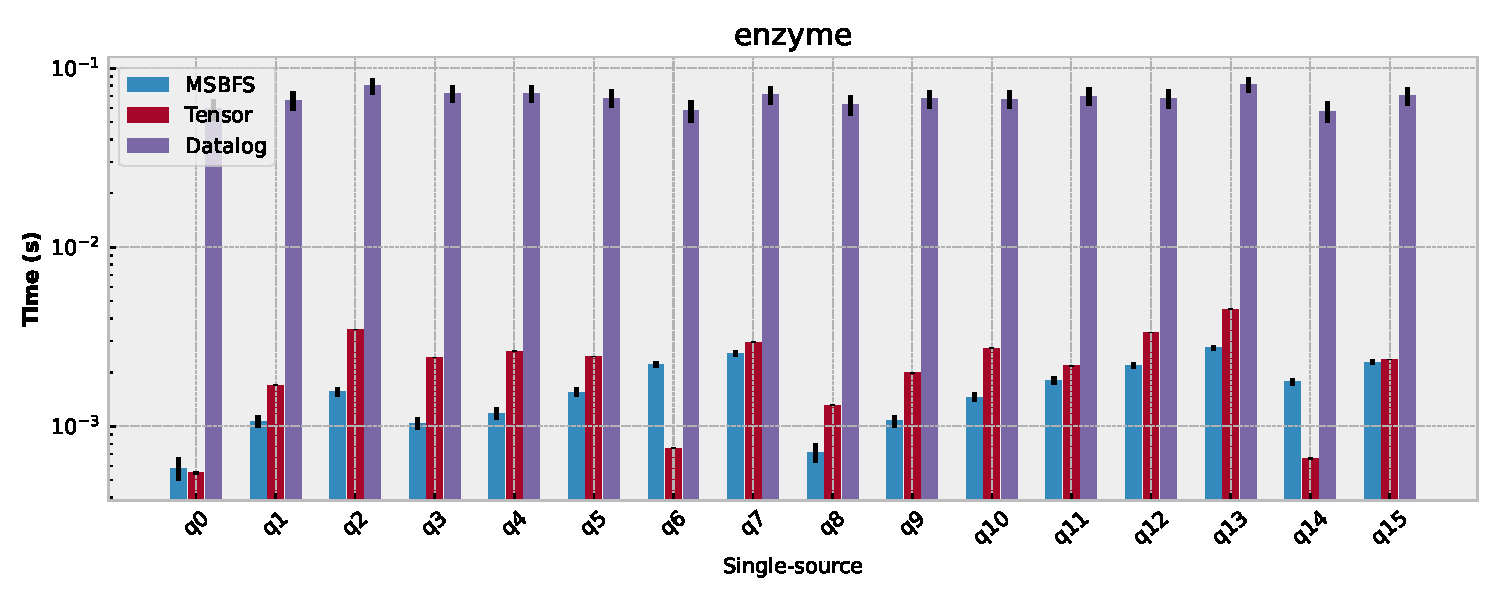
\includegraphics[width=120mm]{pictures/enzyme_ss.pdf} & 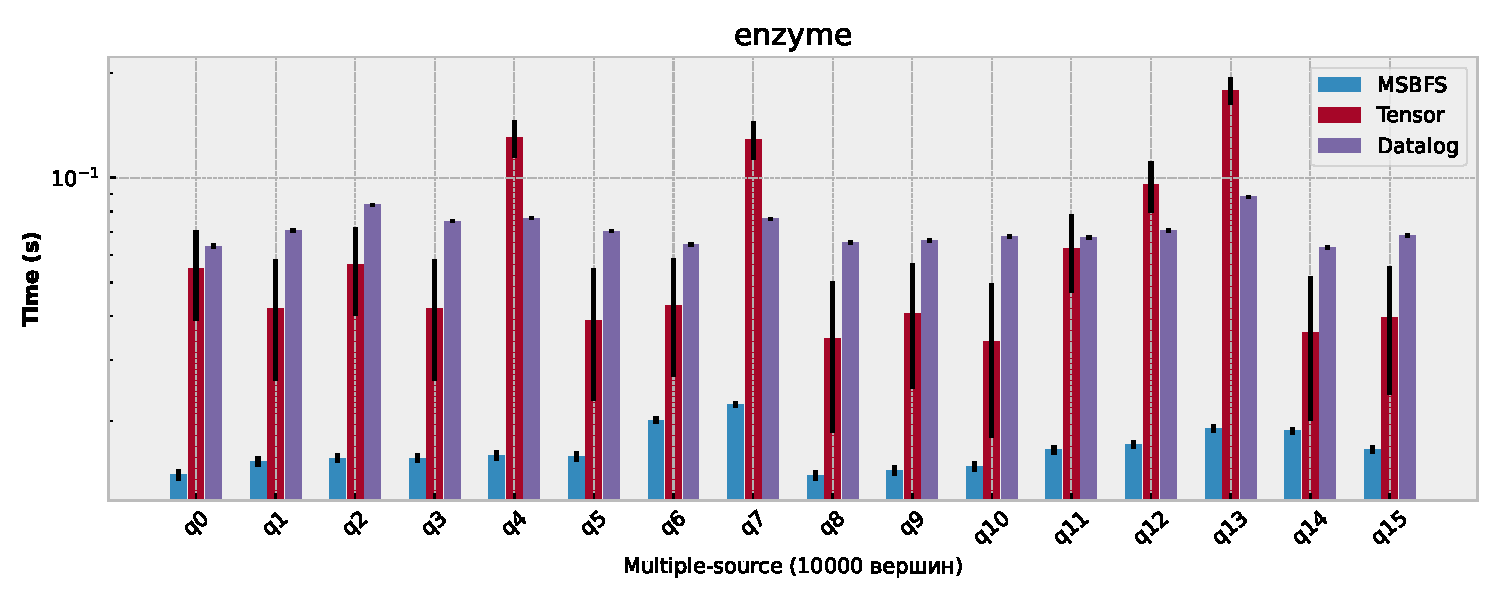
\includegraphics[width=120mm]{pictures/enzyme_ms10000.pdf} \\
                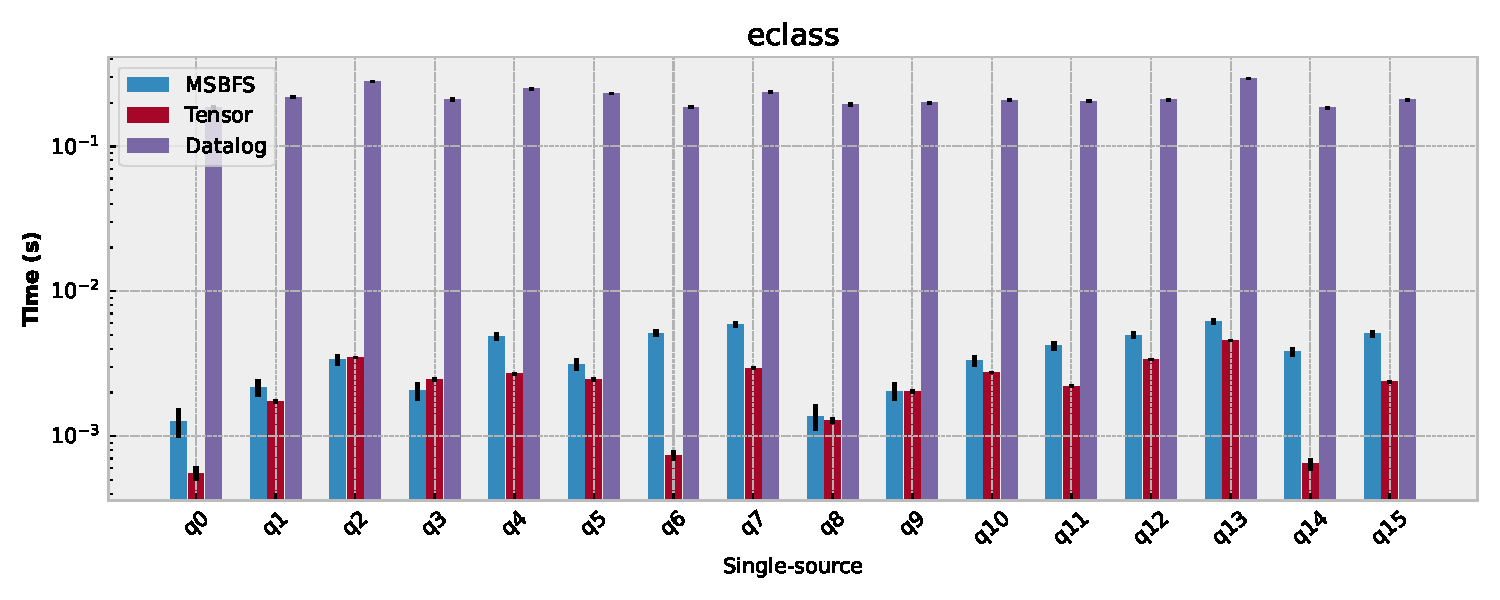
\includegraphics[width=120mm]{pictures/eclass_ss.pdf} & 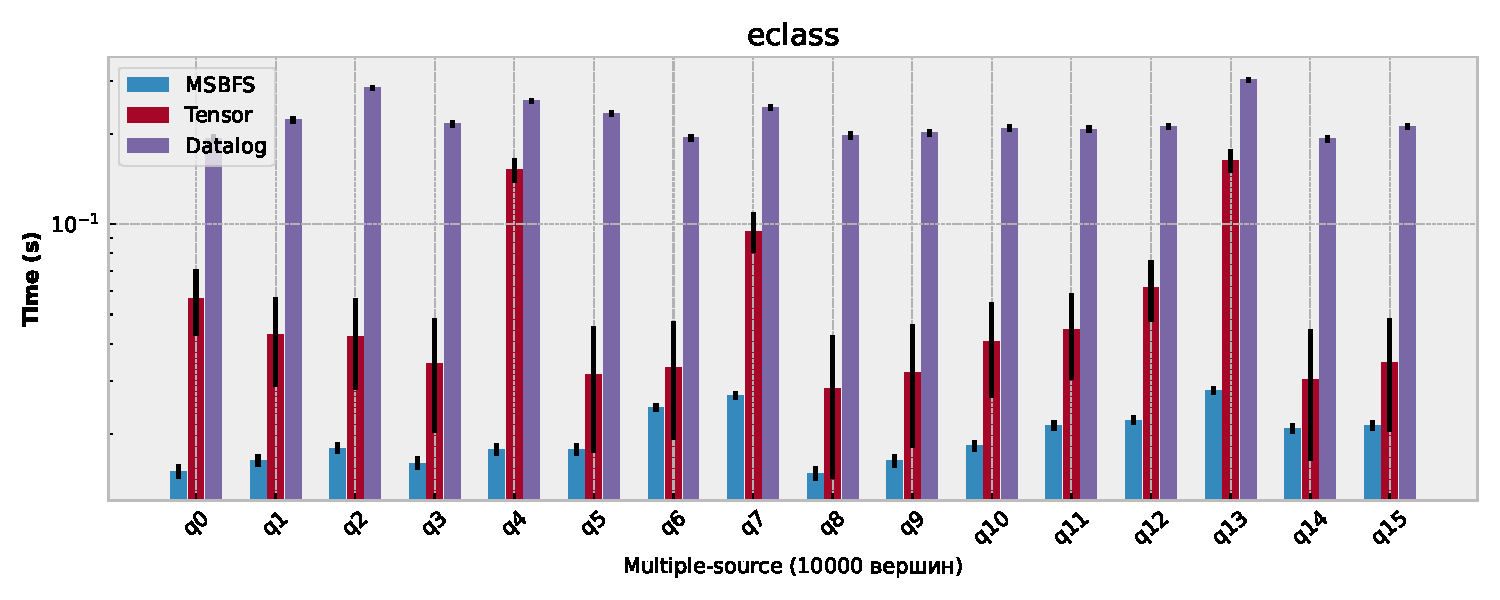
\includegraphics[width=120mm]{pictures/eclass_ms10000.pdf} \\
                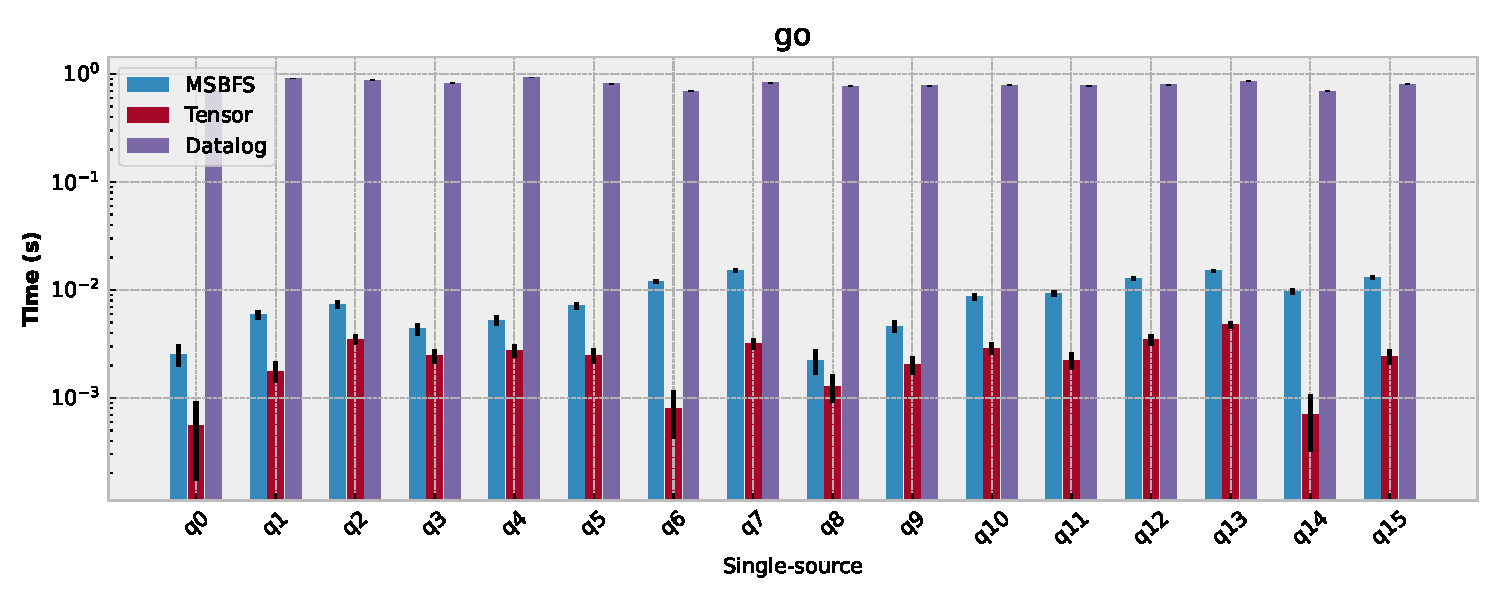
\includegraphics[width=120mm]{pictures/go_ss.pdf}     & 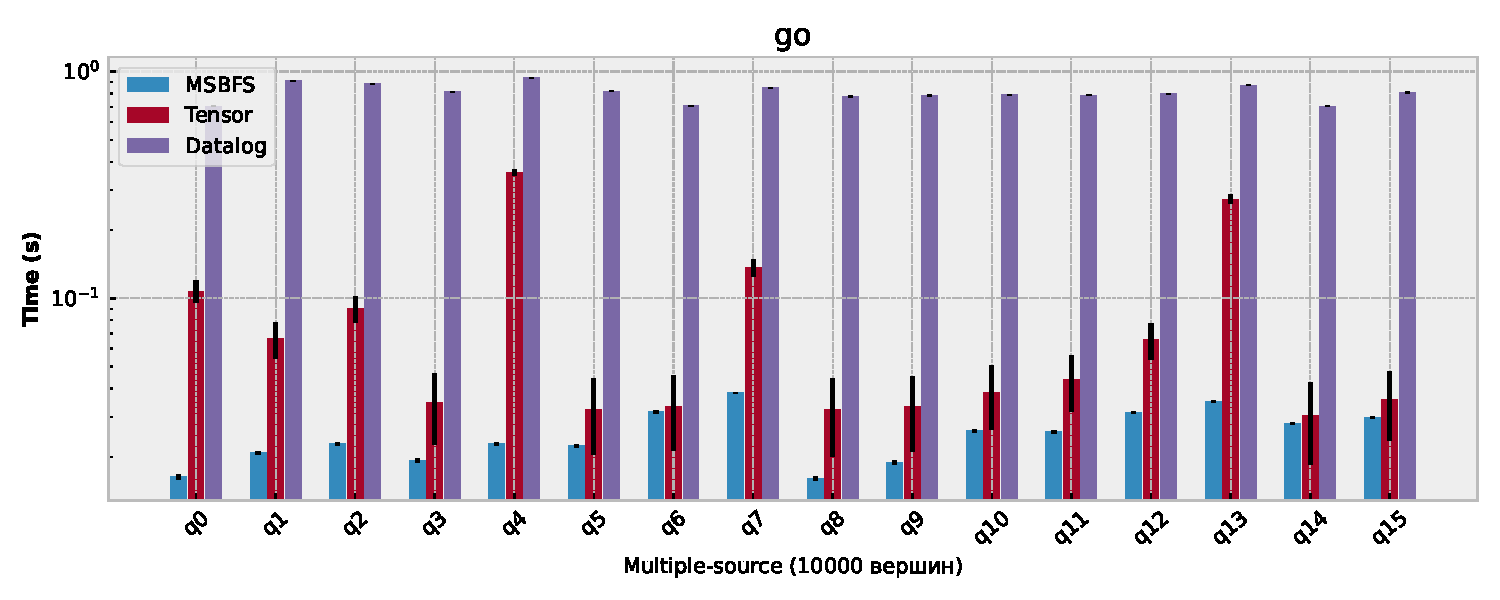
\includegraphics[width=120mm]{pictures/go_ms10000.pdf}     \\
            \end{tabular}
            \caption{Результаты эксперимента на наборе RDF-данных для single-source и multiple-source (10000 вершин) запросов.}
        \end{figure}
    \end{landscape}
    \clearpage
}

% !TeX spellcheck = ru_RU
% !TEX root = vkr.tex

\afterpage{
    \clearpage
    \thispagestyle{empty}
    \begin{landscape}
        \centering
        \begin{figure}
            \begin{tabular}{cc}
                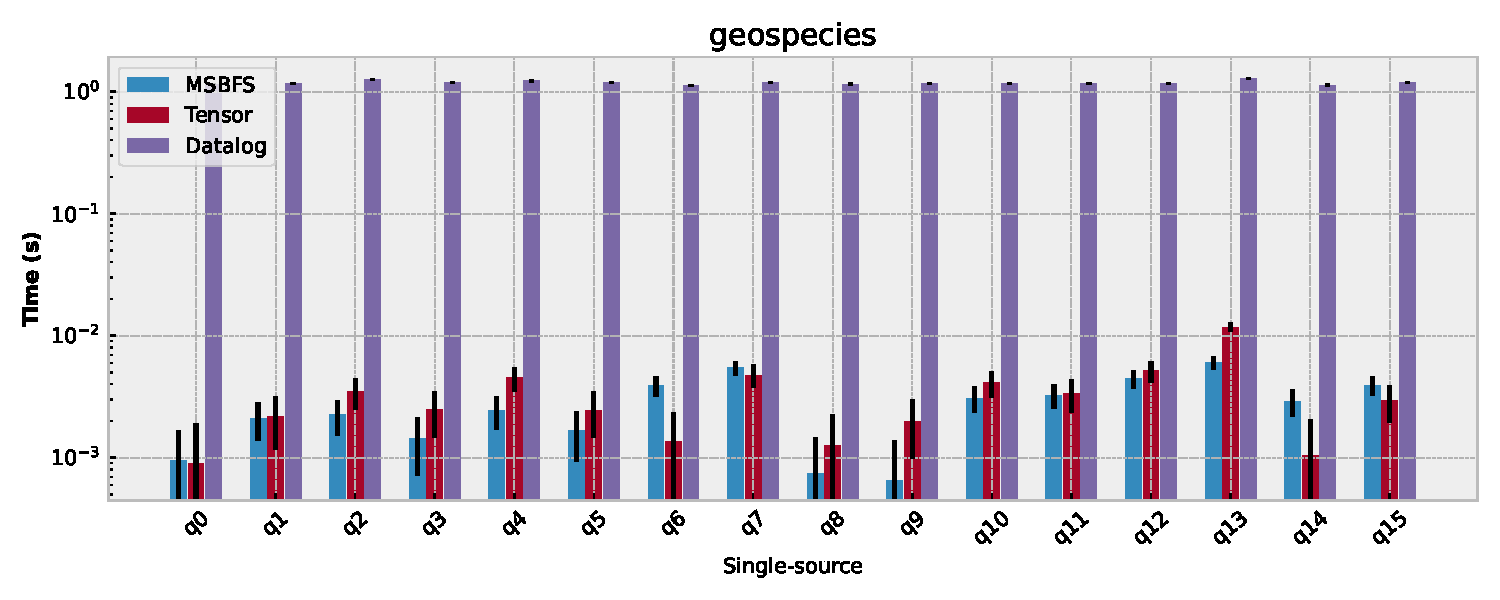
\includegraphics[width=120mm]{pictures/geospecies_ss.pdf} & 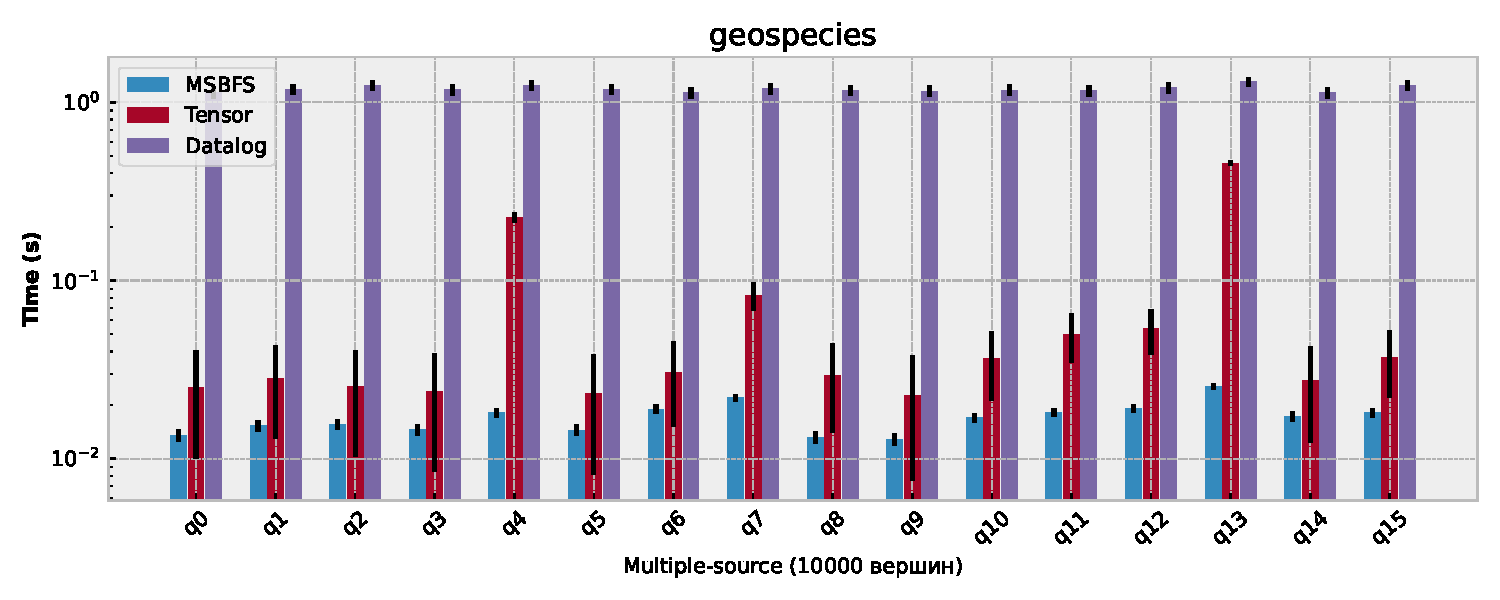
\includegraphics[width=120mm]{pictures/geospecies_ms10000.pdf} \\
                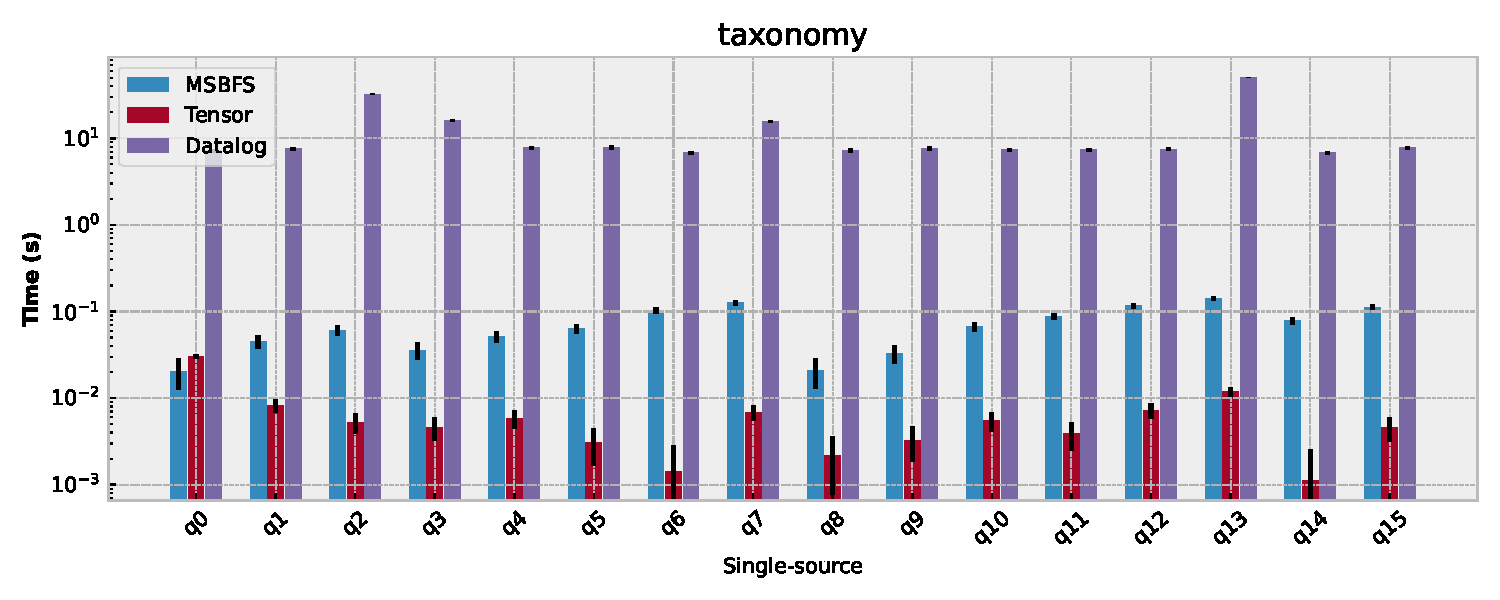
\includegraphics[width=120mm]{pictures/taxonomy_ss.pdf}   & 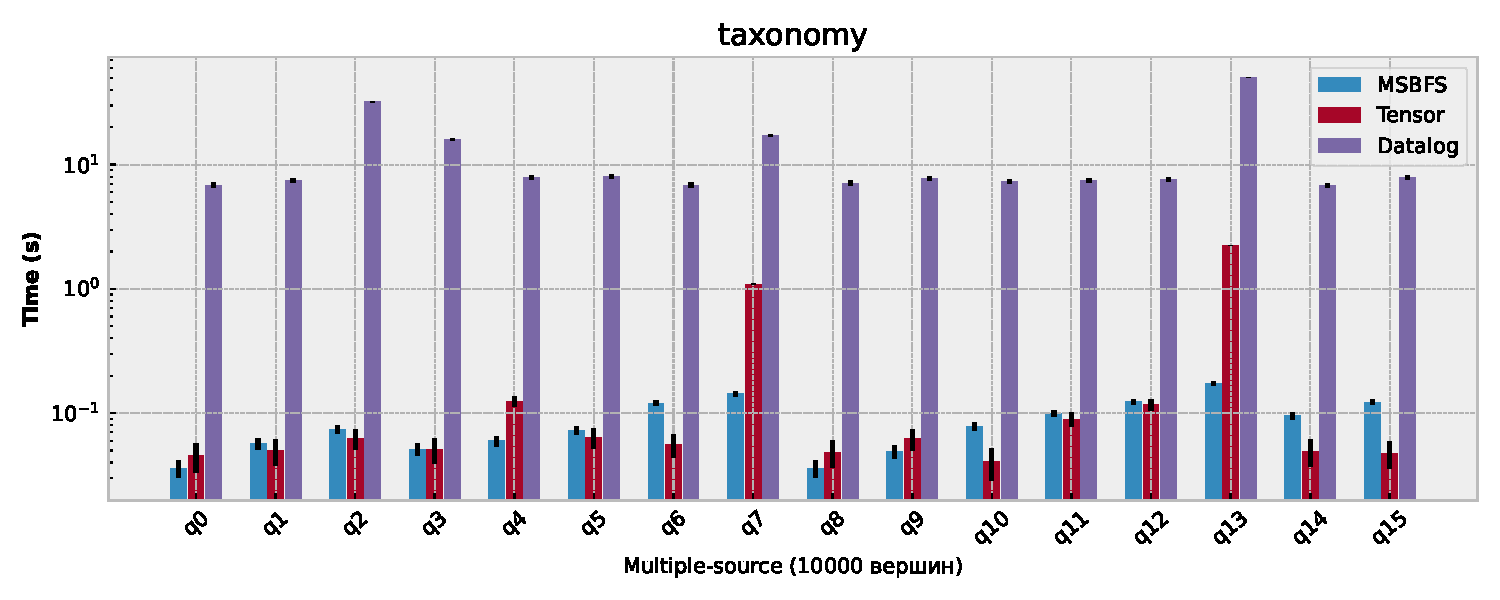
\includegraphics[width=120mm]{pictures/taxonomy_ms10000.pdf}   \\
            \end{tabular}
            \caption{Результаты эксперимента на наборе RDF-данных для single-source и multiple-source (10000 вершин) запросов.}
        \end{figure}
    \end{landscape}
    \clearpage
}


\textbf{RQ2}: Как влияет размер множества стартовых вершин на производительность реализации разработанного алгоритма?

\begin{figure}
    \begin{tabular}{cc}
        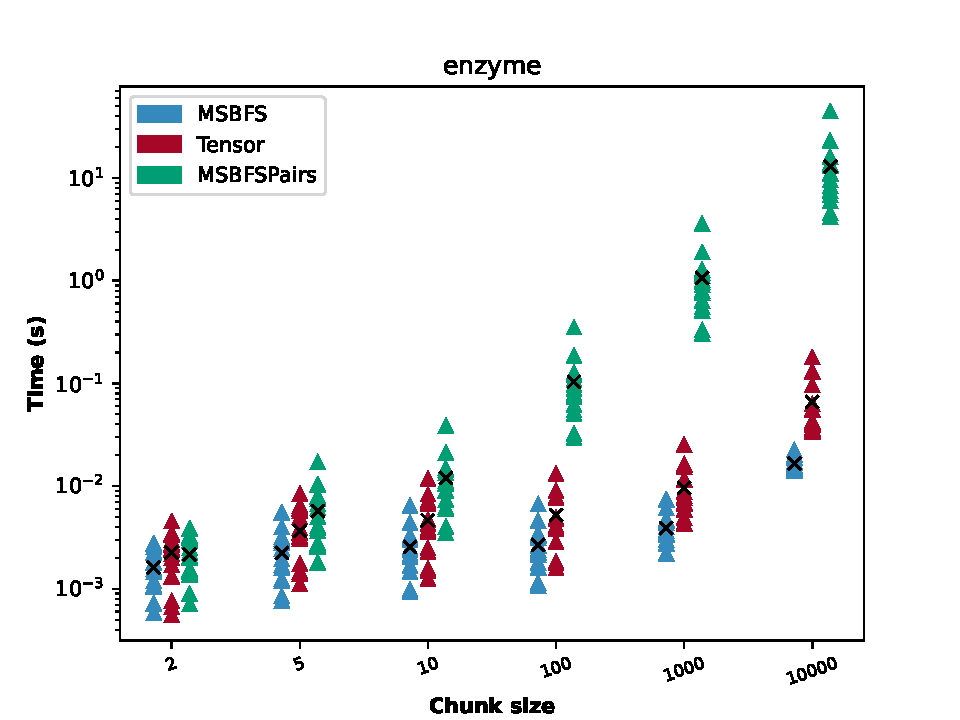
\includegraphics[width=85mm]{pictures/chunks-enzyme.pdf}     & 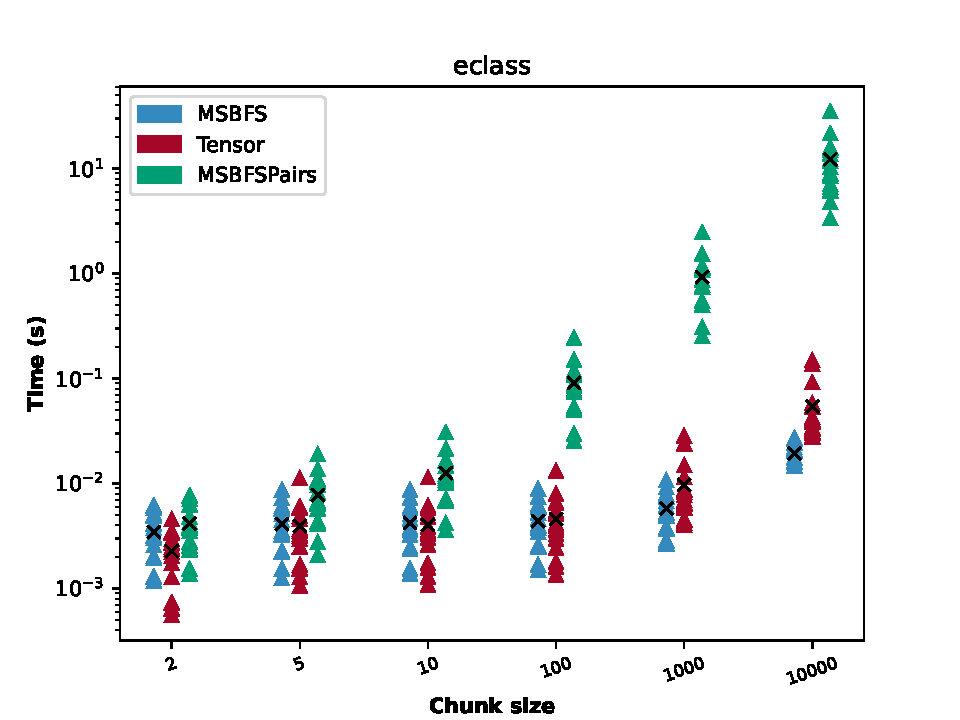
\includegraphics[width=85mm]{pictures/chunks-eclass.pdf}   \\
        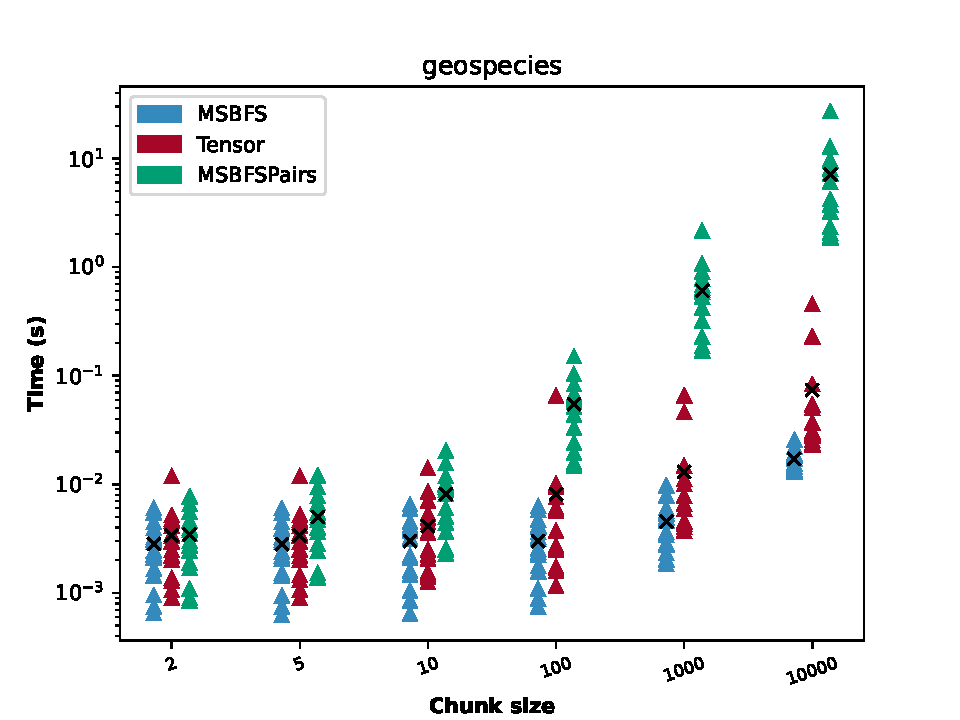
\includegraphics[width=85mm]{pictures/chunks-geospecies.pdf} & 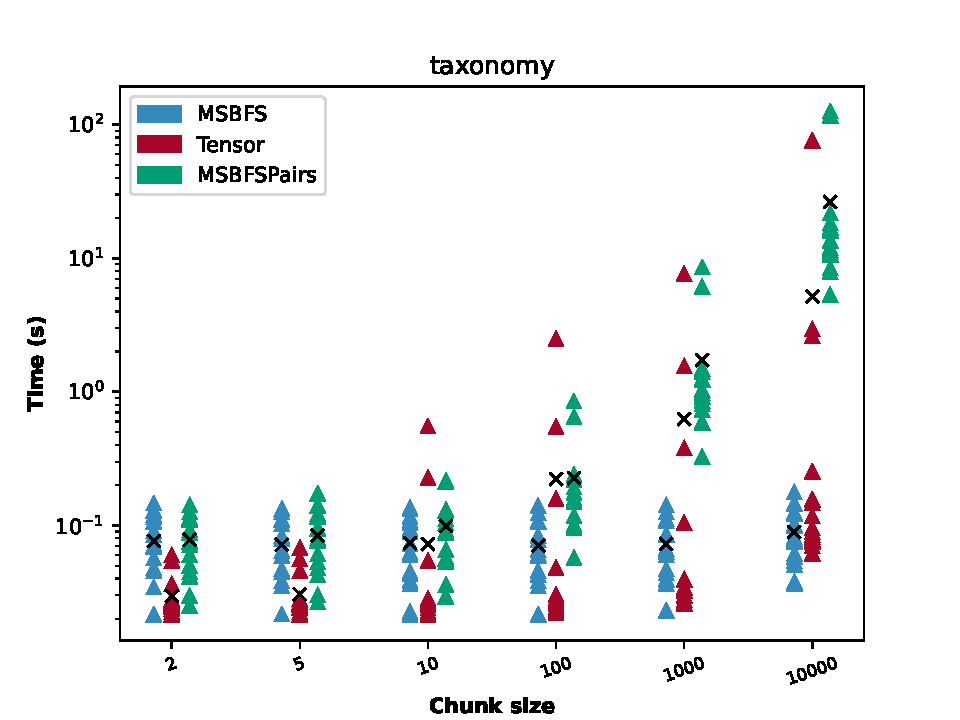
\includegraphics[width=85mm]{pictures/chunks-taxonomy.pdf} \\
        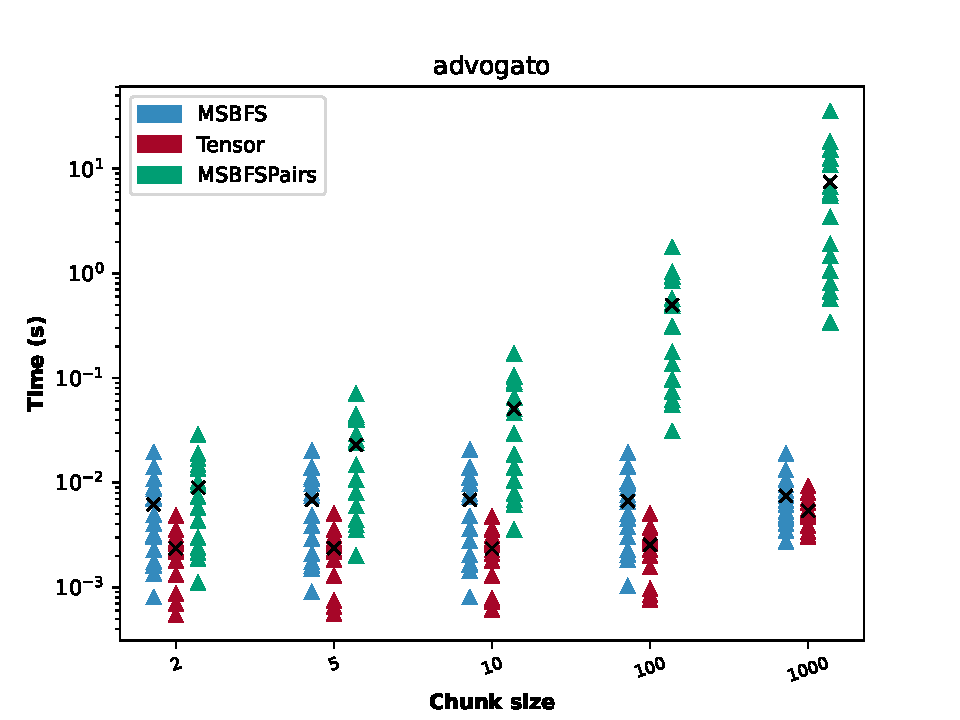
\includegraphics[width=85mm]{pictures/chunks-advogato.pdf}   & 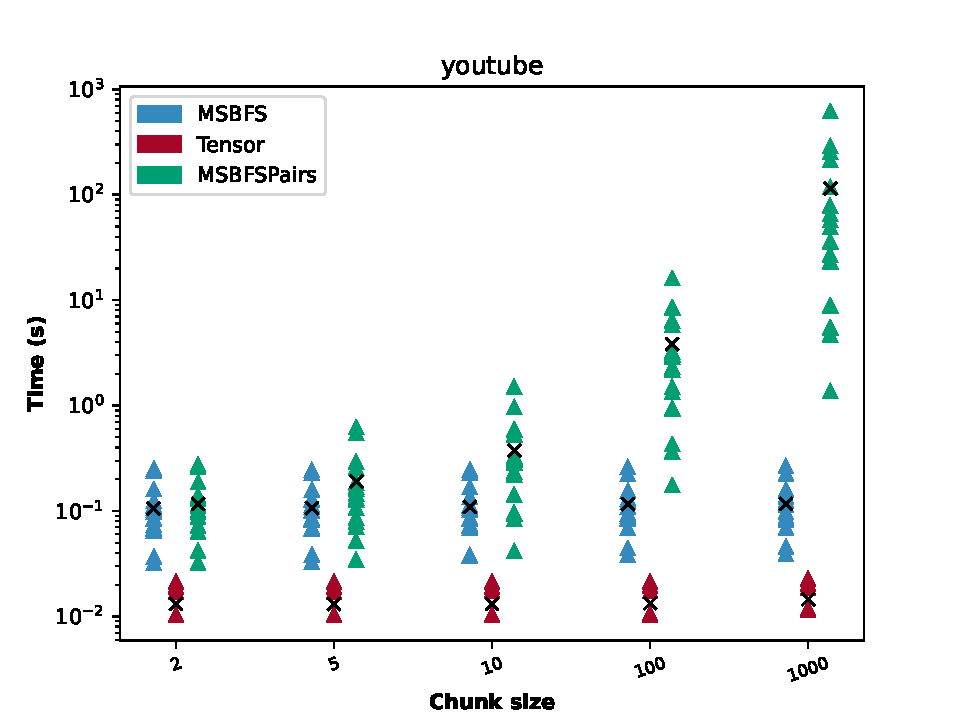
\includegraphics[width=85mm]{pictures/chunks-youtube.pdf}  \\
    \end{tabular}
    \caption{Результаты эксперимента с multiple-source запросами для разных выборок стартовых вершин.}
\end{figure}\label{chunks_bfs_vs_tensor}

Результаты эксперимента по анализу производительности алгоритма для различного числа стартовых вершин представлены на рисунке~\ref{chunks_bfs_vs_tensor}. На нем изображена зависимость времени исполнения запроса от числа стартовых вершин в графе для алгоритмов MSBFS и Tensor. Для выявления зависимости числа стартовых вершин ко времени исполнения была взята еще одна реализация MSBFS, обозначенная MSBFSPairs, которая, в отличие от MSBFS, находит не множество достижимых вершин, а пары начальная--конечная вершина. Основной особенностью этой реализации является то, что инициализация матриц стартовыми вершинами увеличивает размер перемножаемых матриц в $n$ раз, где $n$ --- число стартовых вершин. Это позволяет запомнить от какой стартовой вершины была достигнута каждая из вершин в конечном множестве достижимых. Отмечено время исполнения каждого из запросов, а также выделено среднее время их исполнения. Результаты показывают, что с ростом числа стартовых вершин время работы алгоритма MSBFS меняется несущественно. Это может объясняться тем, что инициализация матриц стартовыми вершинами в его реализации не влияет на размер перемножаемых матриц, что не создает дополнительных расходов во время работы алгоритма, в то время как алгоритмы Tensor и MSBFSPairs страдают от существенного снижения производительности при росте числа стартовых вершин.

Также, на основе этого рисунка можно сделать вывод о том, что время исполнения запроса зависит не только от размера графа, но и от его структуры и разреженности. Так, по анализу данных социальных сетей можно сделать вывод о том, что алгоритм на основе тензорного произведения демонстрирует лучшую производительность для более плотных графов, таких как \textit{advogato} и \textit{youtube}. Именно эти графы имеют наименьшее число различных меток, граф \textit{youtube} также имеет наибольшее число ребер среди всех графов датасета при существенно меньшем числе вершин. Это приводит к тому, что алгоритму, основанному на поиске в ширину, приходится выполнять больше шагов во время обхода графа, так как на этих графах с каждым шагом алгоритма более вероятно увеличение фронта обхода.

Результаты анализа экспериментального исследования позволяют заключить, что реализация алгоритма, основанного на поиске в ширину, показывает приемлемую производительность и во многих случаях работает быстрее, чем реализации аналогов. Более того, реализация алгоритма MSBFS для нахождения всего множества достижимых вершин показывает несущественное ухудшение производительности с ростом числа стартовых вершин. В то же время, реализация алгоритма MSBFSPairs, результатом которого является множество пар начальная--конечная вершина, показала худшие временные характеристики. Более того, заметным является падение производительности обоих реализаций MSBFS на графах социальных сетей, что может быть исследовано в дальнейшем на более широком наборе данных.
